\section{Variações da árvore de Fenwick}

\begin{frame}[fragile]{\it{Range update, point query}}

    \begin{itemize}
        \item Em sua proposta original a árvore de Fenwick responde \textit{queries} no 
            intervalo $[i, j]$ e atualiza os valores em pontos $i$

        \item É possível somar um valor fixo $k$ em todos os elementos $a_k$ cujos índices estão 
            no intervalo $[i, j]$ (\textit{range update}) com complexidade $O(\log N)$

        \item Para isso é necessário reinterpretar os nós da árvore de Fenwick de tal forma
            que o elemento $t_k$ armazenará um valor $x$ que deve ser adicionado a todos
            os elementos $a_i$ tais que $i\geq k$

        \item Assim, uma atualização \code{c}{update(i, j, k)} será feita por meio de duas
            soma pontuais: \code{c}{add(i, k)} e \code{c}{add(j + 1, -k)}

        \item O efeito desta atualização é apresentado abaixo:
        \[
            \ldots, a_{i - 1}, a_i + k, a_{i + 1} + k, \ldots, a_{j - 1} + k,
                a_j + k, a_{j + 1}, \ldots
        \]
    \end{itemize}

\end{frame}

\begin{frame}[fragile]{\it{Range update, point query}}

    \begin{itemize}
        \item Para determinar o valor do elemento $a_i$, é preciso
            fazer uma RSQ deste o início até o ponto $i$

        \item Em notação matemática,
        \[
            a_i = RSQ(1, i) = \sum_{k = 1}^i t_k
        \]

        \item Deste modo, a \textit{query} retorna o valor de um único ponto
            (\textit{point query})

        \item É possível combinar \textit{range updates} com \textit{range queries},
            usando-se duas árvores de Fenwick
    \end{itemize}

\end{frame}

\begin{frame}[fragile]{Implementação de {\it range update} com {\it point query}}
    \inputsnippet{cpp}{1}{20}{codes/ft.cpp}
\end{frame}

\begin{frame}[fragile]{Implementação de {\it range update} com {\it point query}}
    \inputsnippet{cpp}{22}{42}{codes/ft.cpp}
\end{frame}

\begin{frame}[fragile]{Fenwick Tree bidimensional}

    \begin{itemize}
        \item É possível estender o conceito de árvore de Fenwick para duas dimensões

        \item Cada nó $t_{r,s}$ da árvore de Fenwick bidimensional armazenará a soma de todos
            os elementos $a_{i,j}$ da matriz $A$ cujos índices pertençam aos intervalos
            $I_r = [r - p(r) + 1, r]$ e $I_s = [s - p(s) + 1, s]$, respectivamente

        \item Esta interpretação permite uma implementação eficiente tanto da rotina de 
            atualização quando da rotina de soma de intervalo

        \item A atualização consiste em somar um valor fixo $v$ no elemento $a_{i,j}$ da matriz

        \item Devem ser atualizados, portanto, todos os intervalos que contenham tal elemento,
            o que pode ser feito com um laço duplo
    \end{itemize}

\end{frame}

\begin{frame}[fragile]{Fenwick Tree bidimensional}

    \begin{itemize}
        \item $RSQ(i, j)$ é a soma todos os elementos no retângulo definido pelos vértices
            opostos $(1, 1)$ e $(i, j)$ e é a extensão natural da rotina $RSQ(i)$ da árvore
            unidimensional

        \item Para se determinar $RSQ(x_m, y_m, x_M, y_M)$, deve-se utilizar o Princípio da
            Inclusão-Exclusão, isto é,
        \begin{align*}
            RSQ(x_m, y_m, x_M, y_M) &= RSQ(x_M, y_M) - RSQ(x_m - 1, y_M) \\
                &- RSQ(x_M, y_m - 1) + RSQ(x_m - 1, y_m - 1)
        \end{align*}
    \end{itemize}
\end{frame}

\begin{frame}[fragile]{Visualização de $RSQ(x_m, y_m, x_M, y_M)$}

    \begin{figure}
        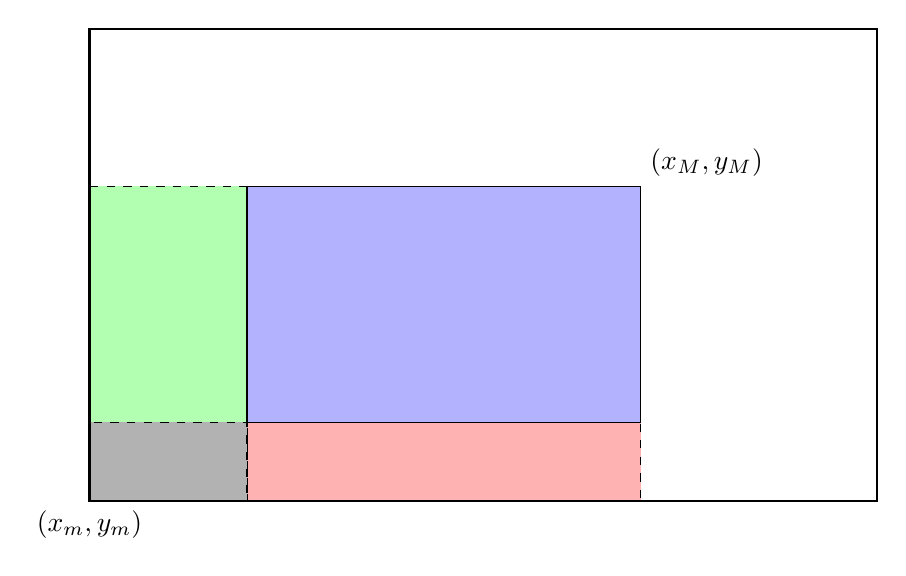
\begin{tikzpicture}
            \draw[dashed,fill=red!30] (0, 0) rectangle (7, 1);
            \draw[dashed,fill=green!30] (0, 0) rectangle (2, 4);
            \draw[dashed,fill=black!30] (0, 0) rectangle (2, 1);
            \draw[fill=blue!30] (2, 1) rectangle (7, 4);
            \draw[thick] (0, 0) rectangle (10, 6);

            \node[anchor=south west] at (7,4) { $(x_M, y_M)$ };
            \node[anchor=north] at (0,0) { $(x_m, y_m)$ };
        \end{tikzpicture}
    \end{figure}

\end{frame}

\begin{frame}[fragile]{Implementação da árvore de Fenwick bidimensional}
    \inputsnippet{cpp}{1}{20}{codes/bit2D.cpp}
\end{frame}

\begin{frame}[fragile]{Implementação da árvore de Fenwick bidimensional}
    \inputsnippet{cpp}{22}{42}{codes/bit2D.cpp}
\end{frame}
